\section{The Dense Baseline}
\label{sec:dense}

This section is told as it happened, because several of its turning points were corrections that ran
against us and the record is only credible if they appear where they occurred.

\subsection{The fair-object rule, and four rehabilitations}

The rule is two-sided: the baseline must be \emph{neither handicapped nor advantaged past the
reference regime}. Concretely, the fact firewall is \textbf{off} (storing facts in weights is
precisely the baseline's job), no memory machinery appears in the graph --- absent, not disabled,
enforced by a source-level import check that is verified red --- and \texttt{loss\_mask=None} is
asserted at the call rather than grepped for.
% fka/dense/, tests/test_dense_baseline.py | M5 §5

% COUNT CONVENTION: the rehabilitation count is the length of the enumerated list
% below, and is matched in the abstract, §1 and Appendix C. Three were chosen; the
% fourth was forced by a defect we found rather than selected (M5 §5.8.1 describes the
% same work as "five, four chosen and one forced" by counting the surface arc as two).
Three were chosen and a fourth was forced.

\paragraph{(i) The recipe audit.} Five arms spanning a 10$\times$ learning-rate range and weight
decay from 0.1 to zero landed \emph{within 0.006 of each other in loss}, and every one sat at the
modal-value baseline storing nothing. The reference's own load-scheduled decay was imported
wholesale with a provenance test. \emph{The recipe is exonerated}; loss separated none of the arms
and corrected accuracy separated all of them from a working model.
% M5 §5.21--5.25

\paragraph{(ii) Token density and the surface arc.} The corpus carried 0.16 bits per token at
character level, so most compute was spent on characters carrying no measured bits. A syllable
surface --- names as a few units from a fixed 608-symbol inventory --- was adopted under a
registered equivalence control. The tokenizer handicap is \emph{real near the cliff}: the surface tax
runs $3.8\times \to 17.1\times \to 26.0\times$, widening as the cliff is approached.
% M5 §5.46
\scope{That tax moved \emph{three} surface coordinates at once (vocabulary, embedding share, tokens
per name), so it is scheme-or-length-or-share and not scheme alone. \S\ref{sec:reconc} shows the
ordering in tokens/name is \emph{non-monotone}, which promotes this scope limit from precaution to
demonstrated. \textbf{Non-license~(2) travels with this claim as well as with the reconciliation}:
the surface term is characterised only over a \emph{measured range} of 2.00--4.15 tokens per name at
matched vocabulary and share, and the verbose surface compared here sits at ${\sim}11$ --- outside
it. This tax is therefore a statement about where \emph{these} two surfaces put the wall, not a
surface coefficient that can be carried to a third.}

\paragraph{(iii) Lexicon accounting.} Vocabulary size is set by the reference's own
$\le 10\%$ embedding-share constraint, not by taste. A correction that added key material to the
sizing denominator was \emph{retired}: a key is presented at query time, so an associative memory
owes bits for the value, not the key --- and the inflated denominator priced the very hypothesis the
sizing was then used to test.
% M5 §5.14

\paragraph{(iv) The ordering leak --- the rehabilitation we did not choose.} The data loader seeded
its shuffle per \emph{template variant}, of which there are five, so at 535 exposures the model saw
\textbf{five permutations of 48{,}000 lines, each ${\sim}107$ times, byte-identical}. A
10M-parameter model memorised the stream instead of the facts. The reading this produced was a
headline in our favour --- \emph{10.86$\times$ the parameters buys no additional addressable keys}
--- and it was an artifact.

The leak was caught by arithmetic, not code review. A statement carries ${\sim}19$ bits of name plus
4.28 bits of value over 14.83 tokens: ${\sim}1.09$ nats/token for a model that predicts structure
and nothing else, and ${\sim}0.89$ for one that additionally knows every value. The 10M model
reported \textbf{0.4157} --- \emph{0.47 nats below the floor for a model that knows everything}.
There is nothing left in the facts to buy that with. Predicted before the fix: remove the repeated
orderings and loss should \emph{rise} to ${\sim}0.89$ while accuracy rises with it. Measured after:
10M \textbf{0.8565}, 1M \textbf{0.9046}, both at the floor, and 10M recall
$\mathbf{4.70\% \to 93.27\%}$.
% M5 §5.63, §5.68

\begin{remark}[Loss carries no verdict information]
The fix \textbf{doubled the loss and multiplied recall twentyfold}, with the same model, seed, steps
and corpus --- only the line order differing. This is the sharpest of five demonstrations that
training loss may not be compared across surfaces, arms or regimes.
\end{remark}

The leak is \emph{capacity-graded, not capacity-gated}: fixing it moved the 1M model
\textbf{+9.7 points} as well. A shortcut some model memorises is also taxing every model that does
not, so every dense number measured before the fix \emph{understates} the baseline.
% M5 §5.67

\subsection{The key-discrimination limit}

\begin{figure}[t]\centering
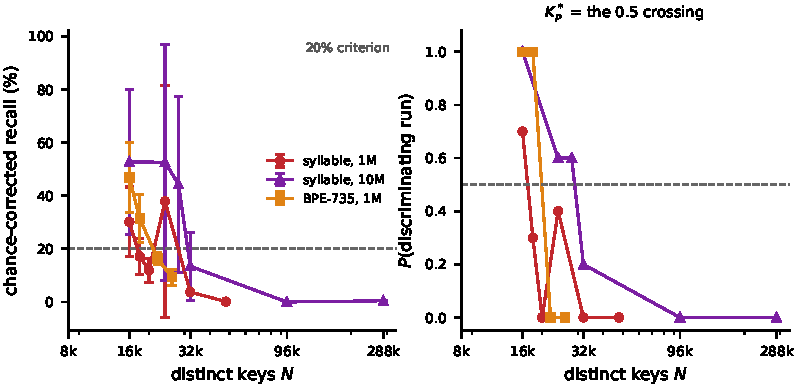
\includegraphics[width=0.98\linewidth]{figures/F5_dense}
\caption{Left: chance-corrected recall against distinct keys, every arm and every seed, with the
20\% criterion marked. Right: $P$(discriminating run), whose 0.5 crossing defines $K^*_P$. Both
panels are parsed from the run logs. \textbf{Seed counts vary by arm and are not interchangeable}
--- syllable 1M: $n = 10, 10, 10, 5, 1, 1$ at $N = 16$k, 18k, 20k, 24k, 32k, 48k; syllable 10M:
$n = 4, 5, 5, 5, 1, 1$ at 16k, 24k, 28k, 32k, 96k, 288k; BPE-735 1M: $n = 5$ at all four arms. The
cliff brackets that define each $K^*_P$ carry the largest samples ($n = 10$ at 1M, $n = 5$ at 10M);
the \textbf{single-seed arms are the two largest at each size}, which sit deep in the dead zone
where every observed seed reads far below criterion, and a $P$ or $\sigma$ read from them would be
uninterpretable. This is the seed table Figure~\ref{fig:frontier} refers to.}
\label{fig:dense}
\end{figure}

The binding constraint is \textbf{discriminable key count, not bits}. Under the honest accounting the
baseline collapses at 0.23--0.49$\times$ load, and a conservative control settles causation: holding
value-load matched while moving keys from 8{,}000 to 16{,}000 drops corrected accuracy from 6.11\% to
2.41\%, monotone across all three relations, with \emph{raw} accuracy rising --- and the control was
given double compute \emph{against} the hypothesis.
% M5 §5.26

\subsection{$K^*$ as a probability object}
\label{sec:kstar}

Single runs cannot locate this transition. Replication at the cliff found seed spreads of
\textbf{72.0 points} at indistinguishable loss ($\sigma_{\text{loss}} = 0.0143$): at 28{,}000 keys,
five seeds gave 0.85\%, 16.55\%, 64.34\%, 66.81\%, 72.86\%.
% M5 §5.118, corrected §5.149.1
The measured object is therefore a probability:

\begin{quote}
$K^*_P$ is the key count at which $P(\text{a training run reaches the 20\% criterion})$ crosses
$0.5$, interpolated log-linearly between bracketing arms, with a minimum of three seeds per point
and five at cliff arms.
\end{quote}

\noindent
$K^*_P(\text{1M}) = \mathbf{16{,}971}$ [16{,}000, 18{,}000], both edges at $n = 10$ on
byte-identical data; $K^*_P(\text{10M}) = \mathbf{28{,}950}$ [28{,}000, 32{,}000] at
$n = 5$.
% M5 §5.128, §5.118

\begin{remark}[A censored statistic ships with the spread it censored --- and with its resolution]
\emph{At $n = 3$}, two arms both read $P = 2/3$ and meant opposite things: at 10M/28{,}000 keys
$\sigma = 39.4$ and the runs were genuinely bimodal; at 1M/18{,}000 keys $\sigma = 5.04$ and the
arm's \emph{mean} simply sat $0.67\sigma$ from the criterion. $P$ discards the margin, so every $P$
is quoted with its $\sigma$.

\emph{Postscript, from replication.} Both arms were later re-run: 10M/28{,}000 reads
$P = \mathbf{0.60}$ at $n = 5$ and 1M/18{,}000 reads $P = \mathbf{0.30}$ at $n = 10$. Neither is
$2/3$, and the pair survives with a second lesson attached. \textbf{At $n = 3$ the standard error of
any proportion is at most $\sqrt{0.25/3} = 0.289$}, so both arms read $2/3 \pm 0.29$ --- a
resolution that cannot separate $0.30$ from $0.60$, which is precisely what they turned out to be.
The original reading was right about the \emph{statistic} and was taken at a sample size that could
not price its own uncertainty. That makes this an instance of the unpriced adjudicator
(Table~\ref{tab:taxonomy}, species 5) as well as of censoring, and the check is one line of
arithmetic that was available on the day the arms ran.
\end{remark}
% M5 §5.149.4

\subsection{Scaling}

\begin{figure}[t]\centering
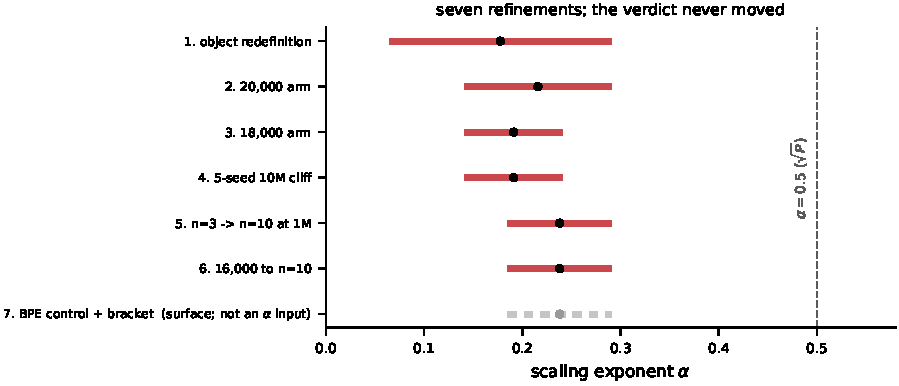
\includegraphics[width=0.62\linewidth]{figures/F8_alpha}
\caption{The $\alpha$ bracket across the seven refinements, labels and brackets loaded from the
ledger (M5 \S5.147). The interval moved --- once \emph{outward}, when a biased $P$ estimate was
corrected --- and the verdict did not. \textbf{Row 7 is drawn hollow because it is not an $\alpha$
input}: $K^*_{\text{BPE}}$ is a surface measurement at 1M that enters the reconciliation, never the
1M/10M ratio, so its interval is carried forward unchanged \emph{by construction} rather than found
unchanged by measurement. The reconstruction of each row's interval from its brackets is checked
against every $\alpha$ value the ledger states outright.}
\label{fig:alpha}
\end{figure}

$\alpha = \mathbf{0.224}$, interval $[\mathbf{0.185}, \mathbf{0.291}]$: a 10.86$\times$ parameter
increase buys 1.71$\times$ more keys. \emph{This is a ratio between two measurements and explicitly
not a fitted law} --- two points cannot discriminate a functional form, and the exponent is reported
as the bracket it is.

\paragraph{Why the ceiling is never approached, stated as the crux.} The best held-out figure the
10M ladder reaches is \textbf{0.075} bits per parameter, against a literature ceiling of
\textbf{2.0}. The gap is not a shortfall in storage: a model at 0.075 has spent almost none of its
bit budget. It is a statement about \emph{which corpora it can be given}. Approaching 2.0 bits per
parameter requires loading a model near its bit capacity, and at 1M parameters that is $N \approx
31{,}686$ --- a key count already far past the measured wall of $K^*_P = 16{,}971$, where recall is
0.34\% and nothing is stored to count. \textbf{Reaching the ceiling requires a load the key wall
forbids.} The two constraints are not independent axes on which a model can be tuned; the second
closes before the first opens, which is why every arm in this study failed at under $0.19\times$ of
its bit capacity rather than at it.

The ledger behind it is seven refinements (Figure~\ref{fig:alpha}): an object redefinition, four
bracket moves, one hostile correction of its own inputs, and the replacement of every $n = 3$
estimate at 1M with an $n = 10$ one. The hostile correction is the instructive entry: taking the
18{,}000 arm from three seeds to ten moved $P$ from $2/3$ to $0.30$ --- the three-seed sample had
caught two of the only three alive values --- and \emph{widened} the interval. More data made the
answer less precise, by correcting a biased input rather than adding a new one.
% M5 §5.125

\subsection{The reconciliation}
\label{sec:reconc}

\begin{figure}[t]\centering
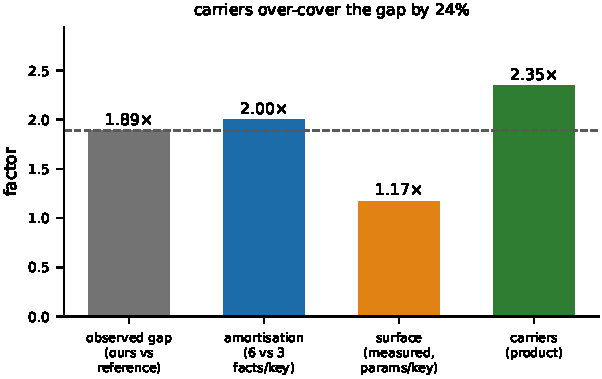
\includegraphics[width=0.55\linewidth]{figures/F6_waterfall}
\caption{The reconciliation. Two measured carriers over-cover the observed gap by 24\%.}
\label{fig:waterfall}
\end{figure}

\begin{table}[t]\centering\small
\caption{The reconciliation in params per key --- the units the claim consumes.}
\label{tab:reconc}
\begin{tabular}{@{}lr@{}}
\toprule
quantity & value \\
\midrule
our params/key, syllable & 55.5 \\
our params/key, BPE & 47.3 \\
the reference's params/key & $\sim$25 \\
\textbf{observed gap} & \textbf{1.89$\times$} \\
\midrule
amortisation (their $\sim$6 facts/key vs our 3) & 2.0$\times$ \\
surface (measured, params/key, 1M) & 1.17$\times$ \\
\textbf{carriers} & \textbf{2.35$\times$} \\
\midrule
\textbf{verdict} & \textbf{RECONCILED} \\
\bottomrule
\end{tabular}

\end{table}

Our regime needs \textbf{55.5} parameters per key \emph{(used-token width,
\S\ref{sec:method})} --- \textbf{47.3} on the better surface --- where the
reference operates at ${\sim}\mathbf{25}$: a gap of $\mathbf{1.89\times}$. Two measured carriers
close it --- amortisation $\mathbf{2.0\times}$ (the reference stores ${\sim}6$ attributes per key
against our 3, read from their configuration) and surface $\mathbf{1.17\times}$ --- for a product of
$\mathbf{2.35\times}$. \textbf{RECONCILED.}

\paragraph{What kind of quantity the amortisation factor is.} It is \emph{not} an empirical estimate
with a hidden error bar. Under the frozen accounting (\S\ref{sec:method}), parameters per
\emph{key} is parameters per \emph{fact} multiplied by facts per key, so a regime storing twice the
attributes behind one key pays half the per-key address cost by \textbf{accounting identity}, not by
measurement. The only input read from the reference's configuration is the \emph{attribute count}
itself --- $\sim$6 against our 3 --- and that is a documented property of their corpus rather than a
fitted parameter. This is what non-license~(1) means when it says the $2.0\times$ is not measured on
our corpus: the \emph{number} comes from their setup, the \emph{entailment} from our accounting, and
neither is an estimate that could have come out otherwise.

\nonlicense{\textbf{The four non-licenses, which travel wherever this is cited.}
\textbf{(1)} The over-coverage is \emph{not slack}: 2.35 against 1.89 means the carriers suffice, not
that either is measured to 24\% accuracy, and amortisation's 2.0$\times$ is read off the reference's
configuration rather than measured on our corpus.
\textbf{(2)} The surface factor holds over the \emph{measured range} 2.00--4.15 tokens per name at
matched vocabulary and share; it is \emph{not} an estimate of the reference's own surface, which
sits at ${\sim}4$ characters per token in a region our synthetic names cannot occupy.
\textbf{(3)} Per-symbol occurrence is a \emph{suspected unmeasured coordinate}, so 1.17$\times$ is a
\emph{net} effect and attributing it to scheme, length or symbol frequency would be smuggling.
\textbf{(4)} 1M only; the BPE arm at 10M is unrun.}

\paragraph{The 40\% lesson.} The surface comparison first produced an \emph{accuracy} ratio of
1.55--1.83$\times$. The reconciliation is stated in params per key, so the caption slot was left
empty until $K^*_{\text{BPE}}$ was measured --- and the key ratio came back at
\textbf{1.17$\times$}. Filling the slot from the quantity we had rather than the one the claim needed
would have overstated the surface term by \textbf{40\%}, in the direction that flatters the
reconciliation.
% M5 §5.137.4, §5.143

\paragraph{Tokens per name is not the surface variable.} Verbose (11 tokens/name) loses to syllable
(2) by 17--26$\times$; syllable loses to BPE (4.15) by 1.55--1.83$\times$ in accuracy. The ordering
is \emph{non-monotone}, so length alone cannot be the mechanism.

\paragraph{One arm was excluded rather than eliminated, and the distinction is the point.} Every
mechanism in Table~\ref{tab:elim} was removed by a measurement or a proof. \textbf{Corpus-trained
BPE merges were removed by neither}: they were ruled out \emph{before any build}, because training
merges on our own rendered corpus lets recurring entity names earn their own merges, whose limit is
one token per name --- entity-atomic, which \emph{deletes} the binding task instead of measuring it.
% M5 §5.82.1
The registered write-up line was to quote the tokens-per-fact such a tokenizer achieves, as the
price of the circularity. \textbf{That line cannot be filled: the arm was never run}, deliberately
and by standing ruling, so no number attaches and none is estimated. It is recorded here as a
registered exclusion rather than as an elimination, because a table whose every other row is a
measurement should not carry one whose evidence column reads ``by design''.

\subsection{Recorded, uninterpreted}

Two observations are recorded without an account, because offering one would exceed what was
measured. First, $\sigma$ \emph{collapses} across the BPE transition ($13.20 \to 8.98 \to 2.33 \to
2.98$) where the syllable surface's rose toward its cliff. Second, per-symbol occurrence differs by
5.2$\times$ between the surfaces (52.6 occurrences per syllable symbol against 275.6 per BPE
fragment at $N = 16{,}000$), which \emph{would} explain the non-monotone ordering --- and is a
post-hoc account whose discriminator, a fourth surface holding one axis fixed while varying the
other, is priced and unrun.
% M5 §5.139
